\documentclass[10pt,a4paper]{article}
\usepackage[utf8]{inputenc}
\usepackage[english]{babel}
\usepackage{amsmath}
\usepackage{amsfonts}
\usepackage{amssymb}
\usepackage{graphicx}
\author{Karl Johan Andreasson \and Josef Sunesson}
\title{Green Elevator}
\begin{document}
\maketitle

\begin{abstract} 
This report handles the implementation of the Green Elevator project in the course Concurrent Programming. The developed controller handles OK.
\end{abstract}

\section{Introduction}
Elevators are present in almost every apartment complex with more than 1 floor. The controller for these elevators has to receive information about the button presses the users make and schedule the elevators accordingly.

To implement this controller to handle the button presses and also the position updates coming from the elevator is the goal of the project. There are several different aspects that has to be considered when scheduling the different elevator cabins. The most important aspects are to minimize waiting time before a cabin comes to serve the user and to minimize the time spent traveling to the desired floor. Another aspect to take into consideration when implementing a scheduling algorithm for the elevator cabins are power consumption.

In the elevator scheduling problem there are hard deadlines to meet once a press of a button has been made. These deadlines are both to not end up with frustrated end users because the controller of the elevators are too slow to schedule the elevators and to not cause the elevators to miss stopping at a floor because the scheduling algorithm was hard at work scheduling another press of a button from a user. To alleviate these problems and to make the solution future proof if the controller should be used with more powerful hardware, a parallelized implementation is desirable.

Another very important aspect of the elevator controller is that it has to provide a fair scheduling of the jobs it receives. No starvation of a job is allowed. Starvation could happen if a job gets postponed because there are other jobs that get scheduled to be executed before and if these jobs continue to arrive the original job is suffering from starvation.

\section{Program outline}
The implementation of the controller of the elevator was made in the language C++ using monitors with locks from the Pthread library for synchronization. C++ was chosen over Java because of the speed increase C++ produces.

The implementation of the elevator controller uses several threads running simultaneously to minimize the response time of the controller. The threads running are one for every elevator car present, one thread that is reading the commands that are coming from the elevators and then dispatching them to either the scheduler or the thread handling the concerned elevator and one last thread to perform scheduling of the jobs.

The threads communicate through monitors and it also through monitors that synchronization is achieved. The choice of monitors was made because of the abstraction it provides. In the implementation there are several monitors present. One for handling jobs that are to be scheduled, one to handle the communication between the controller and the elevators and one for each elevator car. The need of a monitor for communication between the controller and the elevators is because of the choice of implementing the controller in C++ the communication is performed over TCP to the elevators. This forces the communication to be performed serialized and this is performed using a monitor.

\begin{figure}[!h]
\centering
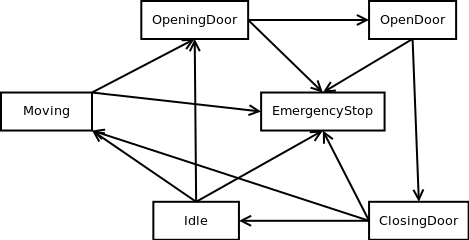
\includegraphics[scale=0.5]{state_transition.png}
\caption{State transitions of an elevator.}
\label{fig:states}
\end{figure}

The elevator is considered as a state machine in the implementation. The states the elevator can have is Idle, Moving, OpeningDoor, ClosingDoor, OpenDoor and EmergencyStop. The state transitions can be found in figure \ref{fig:states}.

A command in the implementation is a button press either inside one of the elevators or on a floor. The command will be read by the reading thread and passed on to the appropriate vector. This vector is either a vector for elevator specific commands for a specific elevator or a vector inside the scheduling monitor for unscheduled commands.

Every handler for the elevators will loop through a while loop until it is signaled by the main thread that the execution is over. Inside the loop it will check for commands to handle inside the elevator specific command vector. These commands are handled inside the monitor associated with the elevator to provide mutual exclusion. Once the commands are handled the elevator invokes a function called run\_elevator inside the elevator monitor, this function will start the elevator if its idle and control close the doors if they are open and the timer has run out. 

\section{Scheduling}
How to decide which elevator that should be sent to handle the command.

\section{Handling commands}

\section{Testing and evaluation}

\section{Conclusion}
\end{document}